% Chapter 1: Introduction - The Fundamental Problem

\section{Introduction}

% The Problem with Words
\begin{frame}{The Fundamental Problem: Computers Don't Understand Words}
\textbf{How do we represent meaning mathematically?}

\begin{columns}
\column{0.5\textwidth}
\textbf{Human Understanding:}
\begin{center}
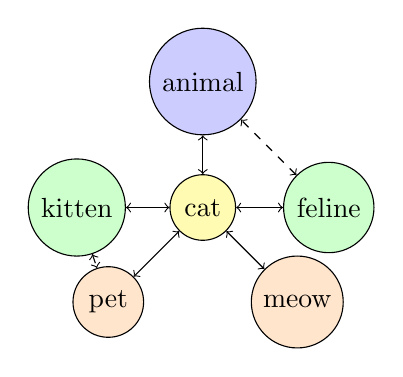
\begin{tikzpicture}[scale=0.8]
    % Central concept
    \node[circle, draw, fill=yellow!30] (cat) at (0,0) {cat};
    
    % Related concepts
    \node[circle, draw, fill=blue!20] (animal) at (0,2) {animal};
    \node[circle, draw, fill=green!20] (kitten) at (-2,0) {kitten};
    \node[circle, draw, fill=green!20] (feline) at (2,0) {feline};
    \node[circle, draw, fill=orange!20] (pet) at (-1.5,-1.5) {pet};
    \node[circle, draw, fill=orange!20] (meow) at (1.5,-1.5) {meow};
    
    % Connections
    \draw[<->] (cat) -- (animal);
    \draw[<->] (cat) -- (kitten);
    \draw[<->] (cat) -- (feline);
    \draw[<->] (cat) -- (pet);
    \draw[<->] (cat) -- (meow);
    \draw[<->, dashed] (kitten) -- (pet);
    \draw[<->, dashed] (feline) -- (animal);
\end{tikzpicture}
\end{center}
Rich semantic connections!

\column{0.5\textwidth}
\textbf{Computer's Dilemma:}
\begin{itemize}
    \item Words are just strings: ``cat'' = ['c','a','t']
    \item No inherent meaning
    \item No similarity measure
    \item Can't do math on strings!
\end{itemize}

\vspace{0.3cm}
\textbf{What We Need:}
\begin{center}
\colorbox{red!10}{\parbox{0.9\columnwidth}{
Convert: ``cat'' $\rightarrow$ [0.2, -0.4, 0.7, ...]\\
Such that: similar words $\rightarrow$ similar vectors
}}
\end{center}
\end{columns}

\vspace{0.3cm}
\textbf{Goal:} Capture meaning in numbers so computers can process language
\end{frame}